% Provenance (never printed): cycle 4 SVT, "La planete Terre": volcanic
% activity, its products and its link with plate boundaries; natural hazards
% and their monitoring; see sources/book1/PROVENANCE.md. Book 1, grade 7,
% chapter 2.
% Vocabulary guard: "magma" first allowed here; "sediment" not before g7.4;
% "subduction zone" is never a term here (gloss: "where one plate sinks under
% another"); "hotspot track" is Book 2's; lahars are called mudflows.
\chapter{Volcanoes}\label{ch:g7:volcanoes}

On 17~May 1980, a geologist stood on a ridge ten kilometres from Mount
St.~Helens, in the north-west of the United States, and took the photograph
on the left below: a smooth, snowy cone, one of the most graceful \omterm{def:g1:landscapes-around-us:landform}{mountains}
of the country. For two months the \omterm{def:g1:landscapes-around-us:landform}{mountain} had been trembling, and its
north side had been swelling outwards like a balloon. The next morning, at
8:32, a small \omterm{def:g4:volcanoes-earthquakes-first-look:earthquake}{earthquake} shook it. The whole swollen side slid away, and
the \omterm{def:g4:volcanoes-earthquakes-first-look:volcano}{volcano} exploded sideways. When the same ridge could be photographed
again, in September, the \omterm{def:g1:landscapes-around-us:landform}{mountain} looked like the photograph on the right.

\begin{omfigure}
\begin{minipage}[b]{0.495\linewidth}\centering
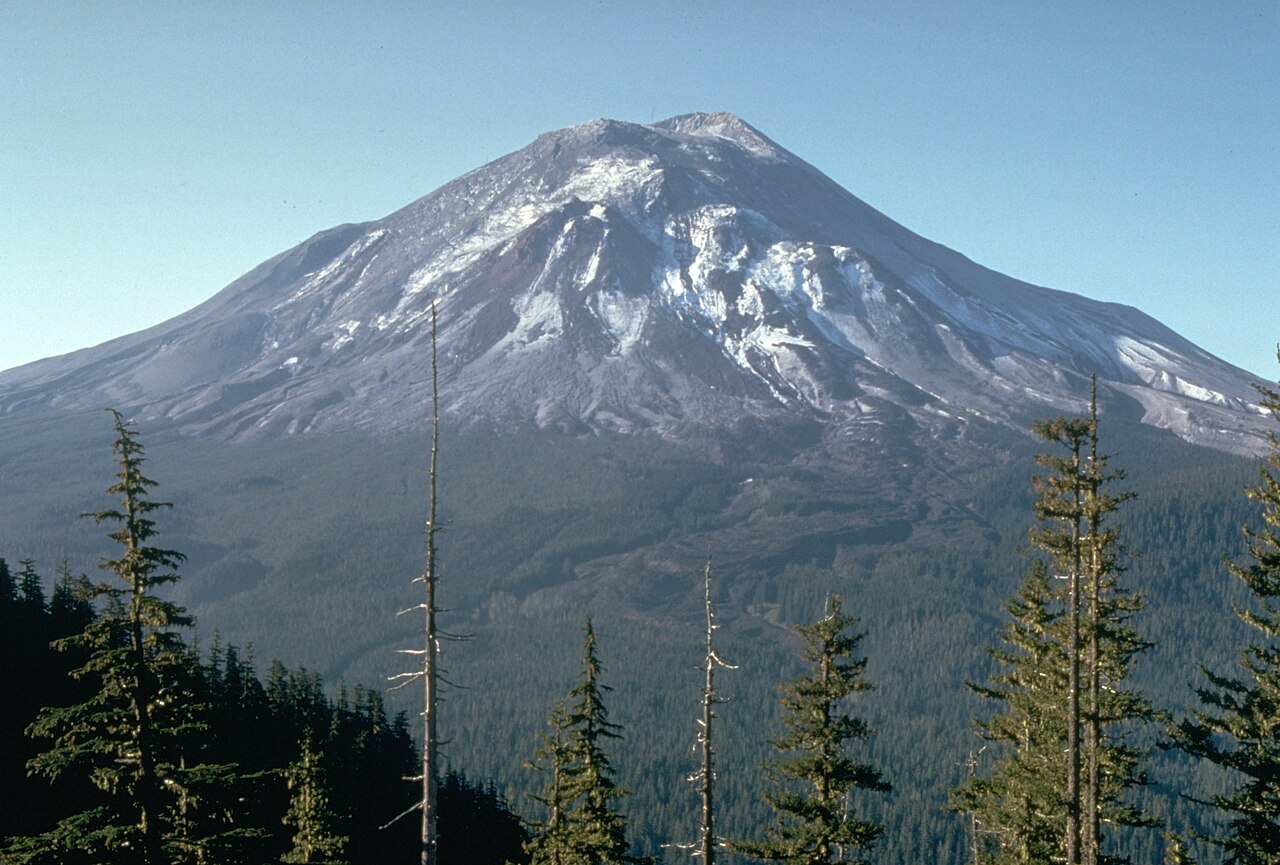
\includegraphics[width=\linewidth]{images/book1/g7-msh-before.jpg}

{\small 17 May 1980, the day before.}
\end{minipage}\hfill
\begin{minipage}[b]{0.495\linewidth}\centering
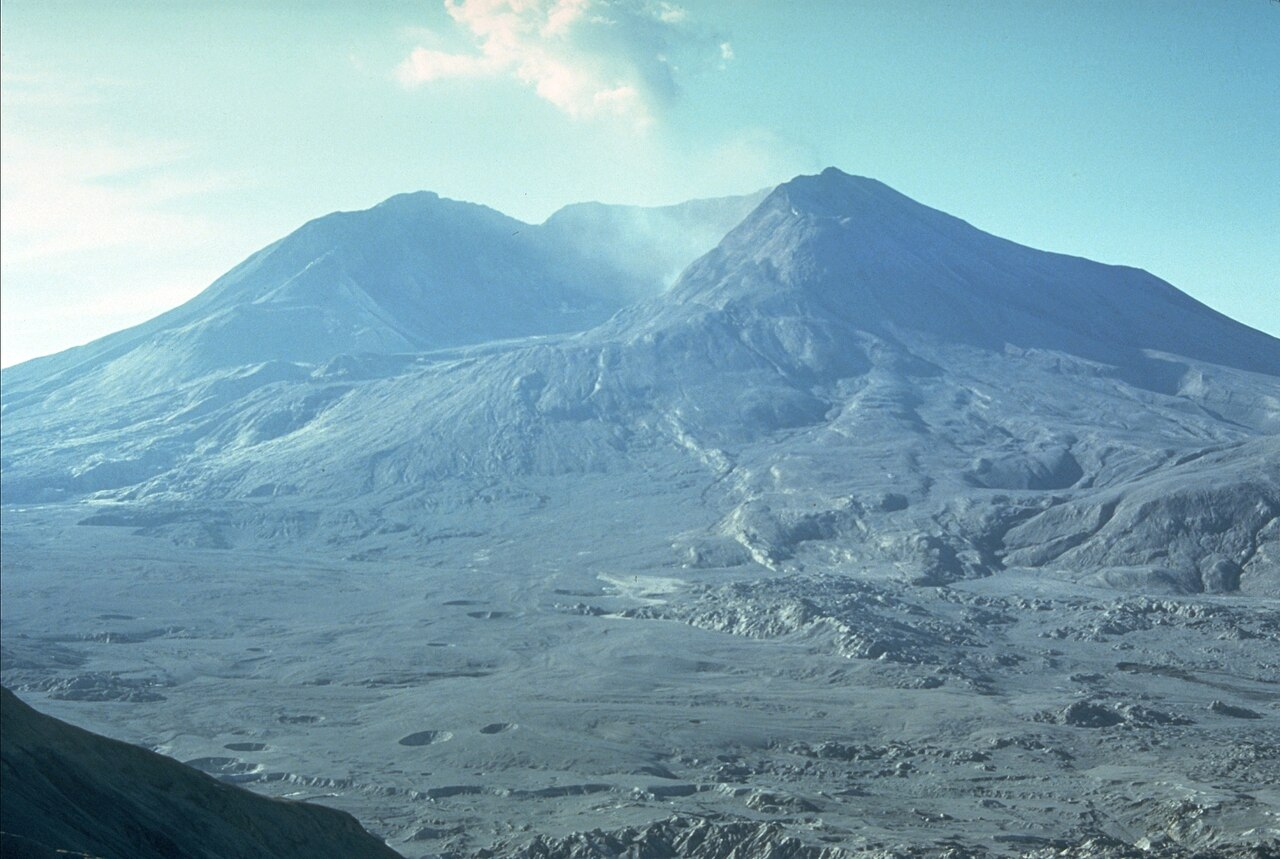
\includegraphics[width=\linewidth]{images/book1/g7-msh-after.jpg}

{\small 10 September 1980.}
\end{minipage}

{\small Mount St.~Helens seen from Johnston Ridge, before and after the
\omterm{def:g4:volcanoes-earthquakes-first-look:eruption}{eruption} of 18~May 1980. The summit and the whole north side are gone; a
\omterm{def:g7:volcanoes:vent}{crater} open to the north has taken their place. Photographs: Harry
Glicken, U.S. Geological Survey (public domain, via Wikimedia Commons).}
% ledger: commons:msh-before, commons:msh-after, usgs:msh-lead-up, usgs:msh-may18
\label{fig:g7:volcanoes:st-helens}
\end{omfigure}

In this chapter we open a \omterm{def:g4:volcanoes-earthquakes-first-look:volcano}{volcano} up, to see what drives an \omterm{def:g4:volcanoes-earthquakes-first-look:eruption}{eruption}; we
find out why some \omterm{def:g4:volcanoes-earthquakes-first-look:volcano}{volcanoes} pour out quiet \omterm{def:g1:landscapes-around-us:water}{rivers} of \omterm{def:g4:volcanoes-earthquakes-first-look:eruption}{lava} while others blow
themselves apart; and we look at the \omterm{def:g3:continents-and-oceans:world-map}{world map} again, to see where the
\omterm{def:g4:volcanoes-earthquakes-first-look:volcano}{volcanoes} are and why.

\begin{recall}
A \emph{\omterm{def:g4:volcanoes-earthquakes-first-look:volcano}{volcano}} is a place where molten \omterm{def:g3:stones-pebbles-sand:rock}{rock} from deep inside the Earth
comes out at the surface, and the \omterm{def:g1:landscapes-around-us:landform}{hill} or \omterm{def:g1:landscapes-around-us:landform}{mountain} that it builds there.
During an \emph{\omterm{def:g4:volcanoes-earthquakes-first-look:eruption}{eruption}} it throws out \omterm{def:g4:volcanoes-earthquakes-first-look:eruption}{lava}, ash and gas
(\cref{ch:g4:volcanoes-earthquakes-first-look}). Below the \omterm{def:g6:inside-the-earth:layers}{crust}, the
\omterm{def:g6:inside-the-earth:layers}{mantle} is made of hot \omterm{def:g3:stones-pebbles-sand:rock}{rock} which is solid, although it can creep very
slowly (\cref{ch:g6:inside-the-earth}). Basalt and granite are \omterm{def:g6:rocks-and-minerals:rock-families}{igneous
rocks}: they form when molten \omterm{def:g3:stones-pebbles-sand:rock}{rock} cools and hardens
(\cref{ch:g6:rocks-and-minerals}). The outer shell of the Earth is broken
into \omterm{def:g7:plate-tectonics:plate}{plates} which move a few centimetres a year; their edges are the \omterm{def:g7:plate-tectonics:plate-boundary}{plate
boundaries} (\cref{ch:g7:plate-tectonics}).
\end{recall}

\section{Inside a volcano}

The \omterm{def:g6:inside-the-earth:layers}{mantle} is solid. Yet in a few places, deep under the surface, a small
part of the \omterm{def:g3:stones-pebbles-sand:rock}{rock} melts. The molten \omterm{def:g3:stones-pebbles-sand:rock}{rock} is lighter than the solid \omterm{def:g3:stones-pebbles-sand:rock}{rock}
around it, so it rises slowly, squeezing up through cracks, like a drop of
oil rising through water.
% ledger: usgs:hawaii-hotspot (magma lighter than the surrounding rock, rises)

\begin{definition}[Magma]\label{def:g7:volcanoes:magma}
\emph{Magma}\index{magma} is molten \omterm{def:g3:stones-pebbles-sand:rock}{rock} underground. It is a hot liquid
which may also carry crystals and, dissolved in it, gases such as water
vapour and carbon dioxide. Magma that comes out at the surface is called
\omterm{def:g4:volcanoes-earthquakes-first-look:eruption}{lava}; as it comes out, it loses most of its gas.
\end{definition}

Rising \omterm{def:g7:volcanoes:magma}{magma} often stops on its way, a few kilometres below the surface,
where it gathers in a large pocket. There it waits, sometimes for
centuries, before an \omterm{def:g4:volcanoes-earthquakes-first-look:eruption}{eruption} empties part of it.

\begin{definition}[Magma chamber]\label{def:g7:volcanoes:magma-chamber}
A \emph{magma chamber}\index{magma chamber} is a large space in the \omterm{def:g3:stones-pebbles-sand:rock}{rocks}
under a \omterm{def:g4:volcanoes-earthquakes-first-look:volcano}{volcano}, a few kilometres down, where \omterm{def:g7:volcanoes:magma}{magma} gathers before an
\omterm{def:g4:volcanoes-earthquakes-first-look:eruption}{eruption}.
\end{definition}

\begin{definition}[Vent and crater]\label{def:g7:volcanoes:vent}
A \emph{vent}\index{vent} is an opening at the surface through which \omterm{def:g7:volcanoes:magma}{magma},
gas and ash come out. A \emph{crater}\index{crater} is the bowl-shaped
hollow around a vent, usually at the top of the \omterm{def:g4:volcanoes-earthquakes-first-look:volcano}{volcano}.
\end{definition}

\begin{omfigure}
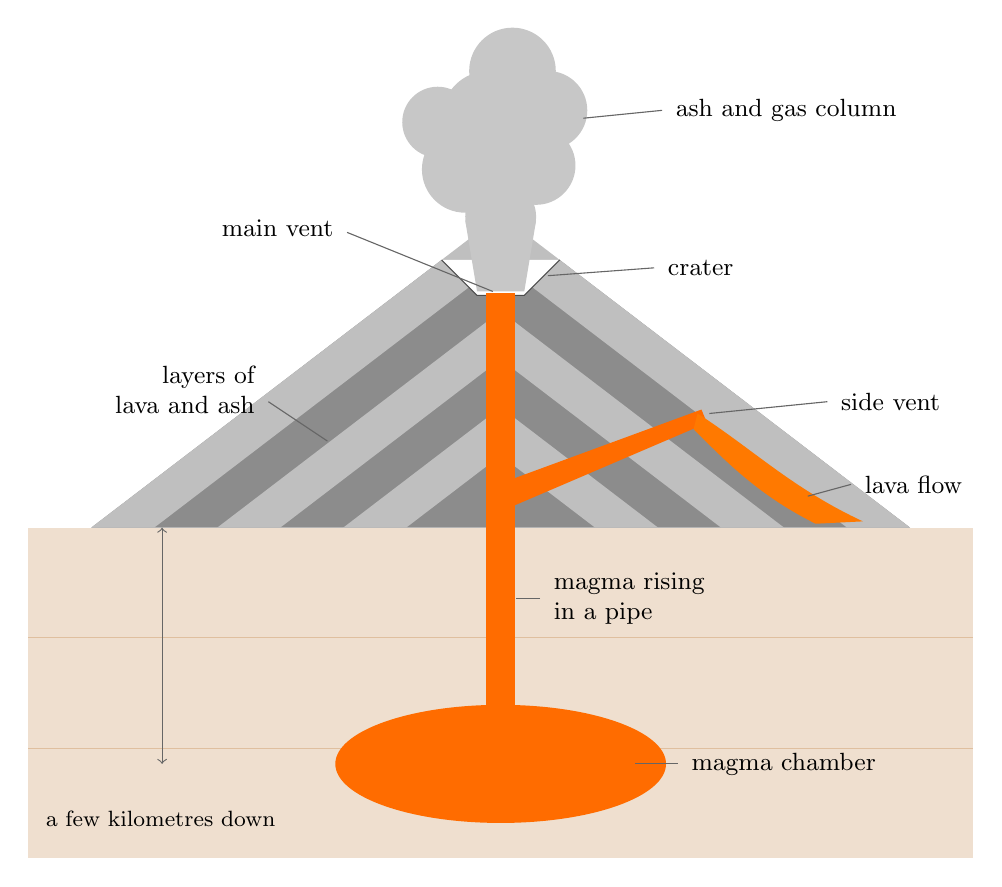
\begin{tikzpicture}[font=\small, x=1cm, y=1cm]
  % rocks below the volcano
  \fill[brown!25] (-6,-4.2) rectangle (6,0);
  \draw[brown!50] (-6,-1.4) -- (6,-1.4) (-6,-2.8) -- (6,-2.8);
  % the cone, built of layers of lava (dark) and ash (light)
  \fill[black!45] (-5.2,0) -- (-0.75,3.4) -- (0.75,3.4) -- (5.2,0) -- cycle;
    % layers dipping outwards, parallel to the flanks (slope 3.4/4.45)
  \foreach \k/\c in {0/black!25, 2/black!25, 4/black!25} {
    \pgfmathsetmacro{\xa}{-5.2+0.8*\k}\pgfmathsetmacro{\xb}{-5.2+0.8*(\k+1)}
    \pgfmathsetmacro{\ya}{(-0.18-\xa)*3.4/4.45}\pgfmathsetmacro{\yb}{(-0.18-\xb)*3.4/4.45}
    \fill[\c] (\xa,0) -- (-0.18,\ya) -- (-0.18,\yb) -- (\xb,0) -- cycle;
    \fill[\c] (-\xa,0) -- (0.18,\ya) -- (0.18,\yb) -- (-\xb,0) -- cycle;
  }
  % the crater at the top
  \fill[white] (-0.75,3.4) -- (-0.3,2.95) -- (0.3,2.95) -- (0.75,3.4) -- cycle;
  \draw[black!70] (-0.75,3.4) -- (-0.3,2.95) -- (0.3,2.95) -- (0.75,3.4);
  % magma chamber and the pipe up to the vent
  \fill[orange!85!red] (0,-3.0) ellipse (2.1 and 0.75);
  \fill[orange!85!red] (-0.18,-2.4) rectangle (0.18,2.98);
  % a side branch to a small side vent
  \fill[orange!85!red] (0.1,0.6) -- (2.55,1.5) -- (2.62,1.33) -- (0.1,0.25) -- cycle;
  % lava flow down the right flank, from the side vent
  \fill[orange!95!red] (2.5,1.45) .. controls (3.2,1.0) and (3.7,0.5) .. (4.6,0.08)
    -- (4.0,0.05) .. controls (3.3,0.4) and (2.9,0.8) .. (2.45,1.25) -- cycle;
  % ash column and gas
    \fill[black!22] (-0.3,3.0) -- (0.3,3.0) -- (0.45,3.9) -- (-0.45,3.9) -- cycle;
  \foreach \x/\y/\r in {0/3.95/0.45, -0.45/4.55/0.55, 0.45/4.6/0.5, -0.15/5.2/0.6,
                        0.6/5.3/0.5, -0.8/5.15/0.45, 0.15/5.8/0.55}
    \fill[black!22] (\x,\y) circle (\r);
  % labels
  \node[anchor=west] at (2.1,5.3) {ash and gas column};
  \draw[black!60] (2.05,5.3) -- (1.05,5.2);
  \node[anchor=west] at (2.0,3.3) {crater};
  \draw[black!60] (1.95,3.3) -- (0.6,3.2);
  \node[anchor=east] at (-2.0,3.8) {main vent};
  \draw[black!60] (-1.95,3.75) -- (-0.1,3.0);
  \node[anchor=west] at (4.2,1.6) {side vent};
  \draw[black!60] (4.15,1.6) -- (2.65,1.45);
  \node[anchor=west] at (4.5,0.55) {lava flow};
  \draw[black!60] (4.45,0.55) -- (3.9,0.4);
  \node[anchor=east, align=right] at (-3.0,1.75) {layers of\\lava and ash};
  \draw[black!60] (-2.95,1.6) -- (-2.2,1.1);
  \node[anchor=west, align=left] at (0.55,-0.9) {magma rising\\in a pipe};
  \draw[black!60] (0.5,-0.9) -- (0.2,-0.9);
  \node[anchor=west] at (2.3,-3.0) {magma chamber};
  \draw[black!60] (2.25,-3.0) -- (1.7,-3.0);
  \node[anchor=west, align=left, font=\footnotesize] at (-5.9,-3.7) {a few kilometres down};
  \draw[black!60, <->] (-4.3,0) -- (-4.3,-3.0);
\end{tikzpicture}

{\small A \omterm{def:g4:volcanoes-earthquakes-first-look:volcano}{volcano} cut open (a drawing, not to scale). \omterm{def:g7:volcanoes:magma}{Magma} gathers in the
\omterm{def:g7:volcanoes:magma-chamber}{magma chamber} and rises through a pipe to the main \omterm{def:g7:volcanoes:vent}{vent}, at the bottom of
the \omterm{def:g7:volcanoes:vent}{crater}; a branch reaches a side \omterm{def:g7:volcanoes:vent}{vent} on the flank. Each \omterm{def:g4:volcanoes-earthquakes-first-look:eruption}{eruption} adds a
layer of \omterm{def:g4:volcanoes-earthquakes-first-look:eruption}{lava} or of ash to the cone.}
\label{fig:g7:volcanoes:cutaway}
\end{omfigure}

So the same molten \omterm{def:g3:stones-pebbles-sand:rock}{rock} has two names. Underground it is \emph{\omterm{def:g7:volcanoes:magma}{magma}}; once
it has come out of a \omterm{def:g7:volcanoes:vent}{vent}, it is \emph{\omterm{def:g4:volcanoes-earthquakes-first-look:eruption}{lava}}. The difference is not only a
matter of words: \omterm{def:g7:volcanoes:magma}{magma} still holds its gas, while \omterm{def:g4:volcanoes-earthquakes-first-look:eruption}{lava} has lost most of it
into the air. We shall see that this gas decides what kind of \omterm{def:g4:volcanoes-earthquakes-first-look:eruption}{eruption} a
\omterm{def:g4:volcanoes-earthquakes-first-look:volcano}{volcano} has.

How hot is it? Scientists of the Hawaiian Volcano Observatory measure the
\omterm{def:g4:volcanoes-earthquakes-first-look:eruption}{lava} as it comes out of the \omterm{def:g7:volcanoes:vent}{vents} of Kilauea, one of the \omterm{def:g4:volcanoes-earthquakes-first-look:volcano}{volcanoes} of
Hawaii: about \qty{1170}{\degreeCelsius}. Hot \omterm{def:g3:stones-pebbles-sand:rock}{rock} glows, and the colour of
the glow depends on its temperature: special cameras read the temperature
of a flow from far away by measuring the colours of its glow. Even the eye
gets a rough idea, as the table shows.
% ledger: usgs:kilauea-temp, usgs:pyrometer

\begin{center}
\small
\begin{tabular}{|l|c|}
\hline
\textbf{colour of the glowing \omterm{def:g3:stones-pebbles-sand:rock}{rock}} & \textbf{temperature} \\
\hline
yellow & about 1000 to \qty{1200}{\degreeCelsius} \\
orange & about 800 to \qty{1000}{\degreeCelsius} \\
red & about 600 to \qty{800}{\degreeCelsius} \\
\hline
\end{tabular}
\end{center}
% ledger: usgs:kilauea-temp

\begin{remark}[A skin that cools in a second]\label{rem:g7:volcanoes:skin}
% ledger: usgs:kilauea-temp
When \omterm{def:g4:volcanoes-earthquakes-first-look:eruption}{lava} first meets the air, its surface cools by hundreds of degrees
every second: a dark skin forms at once on the glowing \omterm{def:g3:stones-pebbles-sand:rock}{rock}. Under the
skin the \omterm{def:g4:volcanoes-earthquakes-first-look:eruption}{lava} stays hot for a long time. In Hawaii, \omterm{def:g4:volcanoes-earthquakes-first-look:eruption}{lava} has flowed in
tunnels under its own hardened roof for \qty{10}{km}, from a \omterm{def:g7:volcanoes:vent}{vent} to the
\omterm{def:g2:water-on-earth:ocean}{sea}, and still reached the shore at about \qty{1140}{\degreeCelsius}: only
about 30~degrees cooler than at the \omterm{def:g7:volcanoes:vent}{vent}.
\end{remark}

\begin{omfigure}
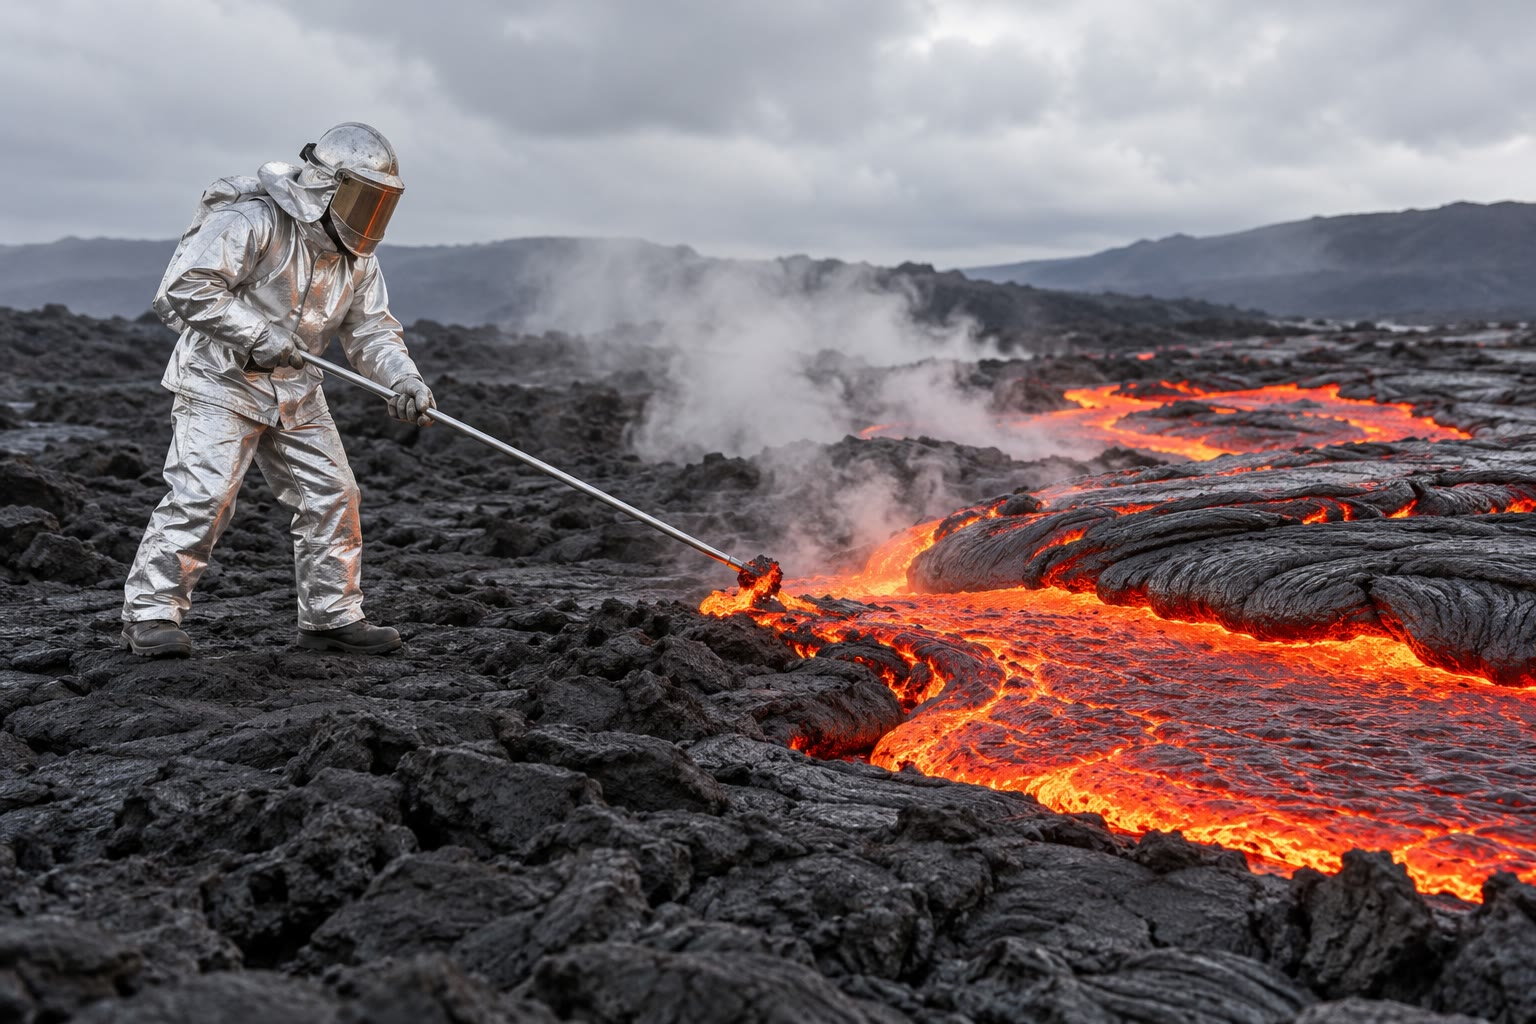
\includegraphics[width=0.6\linewidth]{images/book1/ai/g7-volcanologist.jpg}

{\small A volcanologist in a heat-reflecting suit takes a sample of \omterm{def:g4:volcanoes-earthquakes-first-look:eruption}{lava}
with a long steel pole (AI-generated illustration of a generic scene).
Only trained scientists, with this kind of equipment, go close to flowing
\omterm{def:g4:volcanoes-earthquakes-first-look:eruption}{lava}; everyone else watches from where the authorities allow.}
\label{fig:g7:volcanoes:volcanologist}
\end{omfigure}

\section{Two ways to erupt}

Mount St.~Helens blew itself apart. The \omterm{def:g4:volcanoes-earthquakes-first-look:volcano}{volcanoes} of Hawaii, on the
contrary, usually pour out \omterm{def:g4:volcanoes-earthquakes-first-look:eruption}{lava} which flows away down their slopes.
Geologists sort \omterm{def:g4:volcanoes-earthquakes-first-look:eruption}{eruptions} into two kinds.

\begin{definition}[Effusive and explosive eruptions]\label{def:g7:volcanoes:eruption-types}
In an \emph{effusive eruption}\index{effusive eruption} the \omterm{def:g7:volcanoes:magma}{magma} comes out
quietly as \omterm{def:g4:volcanoes-earthquakes-first-look:eruption}{lava}, which flows away from the \omterm{def:g7:volcanoes:vent}{vent}, sometimes for kilometres,
or spurts up in fountains of glowing drops. In an \emph{explosive
eruption}\index{explosive eruption} the \omterm{def:g7:volcanoes:magma}{magma} is blown to pieces by its
own gas: a column of ash, gas and lumps of \omterm{def:g3:stones-pebbles-sand:rock}{rock} is thrown high into the
sky.
\end{definition}

\begin{omfigure}
\begin{minipage}[t]{0.49\linewidth}\centering
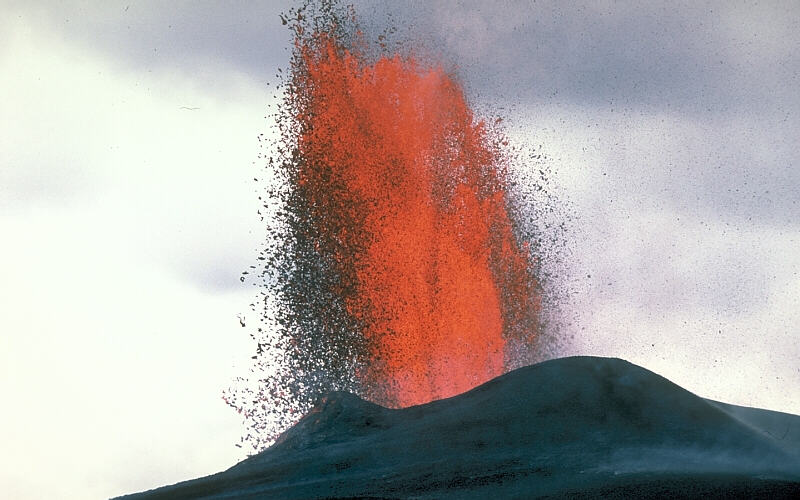
\includegraphics[height=4.5cm]{images/book1/g7-lava-fountain.jpg}

{\small Effusive: a fountain of \omterm{def:g4:volcanoes-earthquakes-first-look:eruption}{lava} at Kilauea, Hawaii, 1983.
Photograph: J.~D. Griggs, USGS.}
\end{minipage}\hfill
\begin{minipage}[t]{0.49\linewidth}\centering
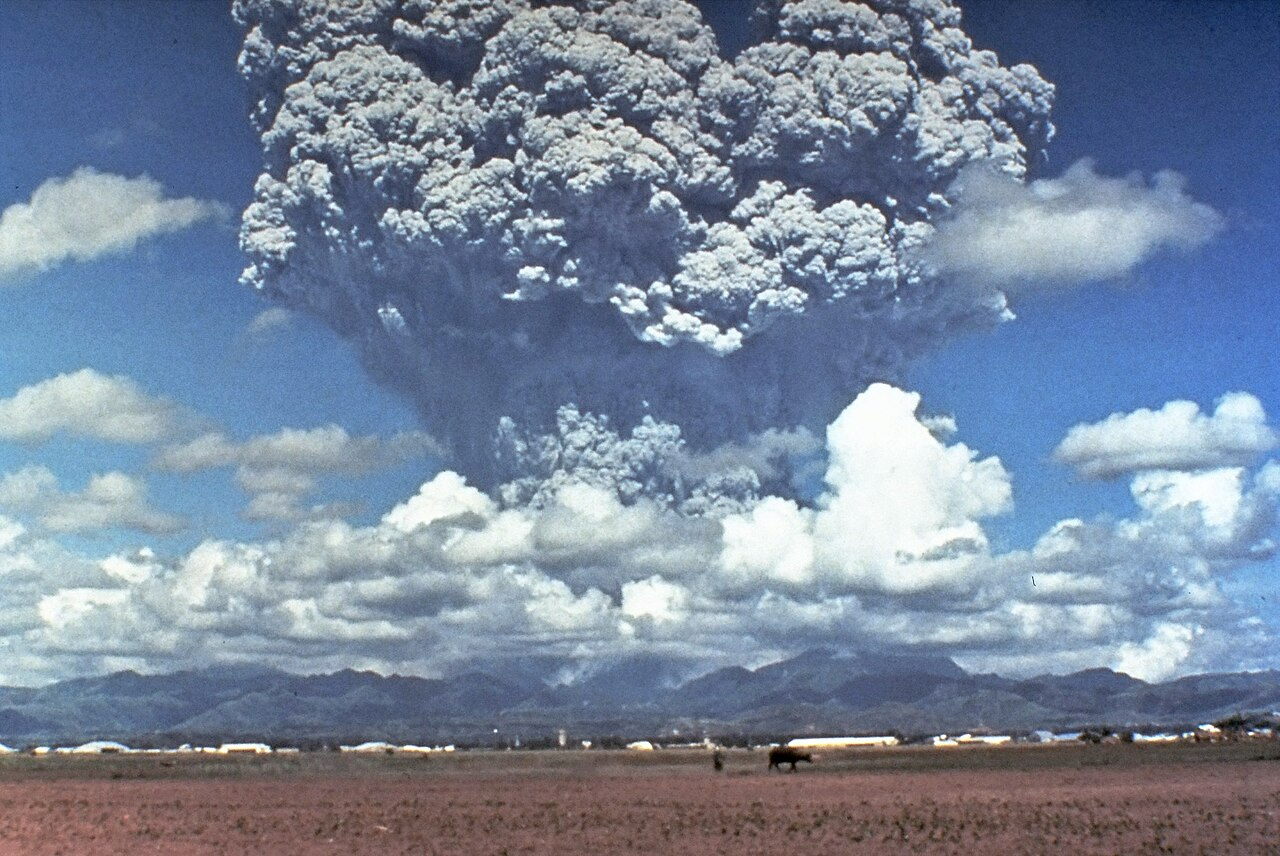
\includegraphics[height=4.5cm]{images/book1/g7-pinatubo.jpg}

{\small Explosive: the \omterm{def:g4:volcanoes-earthquakes-first-look:eruption}{eruption} column of Mount Pinatubo, Philippines,
12~June 1991. Photograph: Dave Harlow, USGS.}
\end{minipage}\par\medskip


{\small Both photographs are in the public domain (via Wikimedia
Commons).}
% ledger: commons:lava-fountain, commons:pinatubo
\label{fig:g7:volcanoes:two-photos}
\end{omfigure}

What makes the difference? Two things: how runny the \omterm{def:g7:volcanoes:magma}{magma} is, and how
much gas it holds.

\textbf{Runny or sticky.} Some \omterm{def:g7:volcanoes:magma}{magma} is runny, almost like warm honey: this
is the case of the \omterm{def:g7:volcanoes:magma}{magma} that cools into dark basalt, as in Hawaii. Other
\omterm{def:g7:volcanoes:magma}{magma} is thick and sticky, like cold honey or toothpaste. Through runny
\omterm{def:g7:volcanoes:magma}{magma}, gas bubbles rise easily and escape at the surface, a few at a time.
In sticky \omterm{def:g7:volcanoes:magma}{magma} the bubbles are trapped.

\textbf{Little or much gas.} A bottle of fizzy water holds a lot of gas
dissolved in the water, kept there by the pressure inside the closed
bottle; you cannot see it. Open the bottle and the pressure drops: bubbles
appear everywhere, and if the bottle has been shaken, the foam bursts out.
\omterm{def:g7:volcanoes:magma}{Magma} deep underground also holds gas dissolved under high pressure. As it
rises, the pressure drops and the gas comes out of solution as bubbles.
% ledger: usgs:volcanic-gases

Put the two together. Runny \omterm{def:g7:volcanoes:magma}{magma} with little gas lets its bubbles go and
comes out as flowing \omterm{def:g4:volcanoes-earthquakes-first-look:eruption}{lava}: the \omterm{def:g4:volcanoes-earthquakes-first-look:eruption}{eruption} is effusive. Sticky \omterm{def:g7:volcanoes:magma}{magma} full of
gas keeps its bubbles until they swell so much that they tear the \omterm{def:g7:volcanoes:magma}{magma}
into shreds: the \omterm{def:g4:volcanoes-earthquakes-first-look:eruption}{eruption} is explosive. The shreds of frothy \omterm{def:g7:volcanoes:magma}{magma} freeze
in the air into ash and into pumice, a \omterm{def:g3:stones-pebbles-sand:rock}{rock} so full of bubbles that it can
float.

\begin{example}[Pinatubo, 1991: the flat soda and the shaken one]\label{ex:g7:volcanoes:pinatubo}
% ledger: usgs:pinatubo-1991
In June~1991 the first \omterm{def:g7:volcanoes:magma}{magma} reached the surface of Mount Pinatubo, in the
Philippines. On its way up it had lost most of its gas, ``like a bottle of
soda pop gone flat'', in the words of the scientists who were watching. It
oozed out slowly and piled up into a mound over the \omterm{def:g7:volcanoes:vent}{vent}: no explosion.
Then, on 12~June, \omterm{def:g7:volcanoes:magma}{magma} still full of gas reached the surface and
exploded --- the column in the photograph above. On 15~June, even more
gas-rich \omterm{def:g7:volcanoes:magma}{magma} arrived, and the \omterm{def:g4:volcanoes-earthquakes-first-look:volcano}{volcano} had one of the largest \omterm{def:g4:volcanoes-earthquakes-first-look:eruption}{eruptions}
of the twentieth century: it threw out more than five cubic kilometres of
\omterm{def:g3:stones-pebbles-sand:rock}{rock} and ash, its ash \omterm{def:g4:clouds-rain-snow:cloud}{cloud} rose \qty{35}{km} high, and the top of the
\omterm{def:g1:landscapes-around-us:landform}{mountain} collapsed into a hollow \qty{2.5}{km} across. The same \omterm{def:g4:volcanoes-earthquakes-first-look:volcano}{volcano},
the same week: the gas made the difference.
\end{example}

The shape of a \omterm{def:g4:volcanoes-earthquakes-first-look:volcano}{volcano} keeps the memory of its \omterm{def:g4:volcanoes-earthquakes-first-look:eruption}{eruptions}. Runny \omterm{def:g4:volcanoes-earthquakes-first-look:eruption}{lava} flows
far before it hardens, so layer after layer it builds a broad \omterm{def:g1:landscapes-around-us:landform}{mountain} with
gentle slopes, shaped like a warrior's shield lying on the ground: a
\emph{shield \omterm{def:g4:volcanoes-earthquakes-first-look:volcano}{volcano}}. Mauna Loa, in Hawaii, is one. Sticky \omterm{def:g4:volcanoes-earthquakes-first-look:eruption}{lava} and ash
pile up close to the \omterm{def:g7:volcanoes:vent}{vent}, into a steep cone made of layers of \omterm{def:g4:volcanoes-earthquakes-first-look:eruption}{lava} and
ash: a \emph{stratovolcano} (\emph{strata} means layers). Mount St.~Helens
and Pinatubo are two of them.

\begin{omfigure}
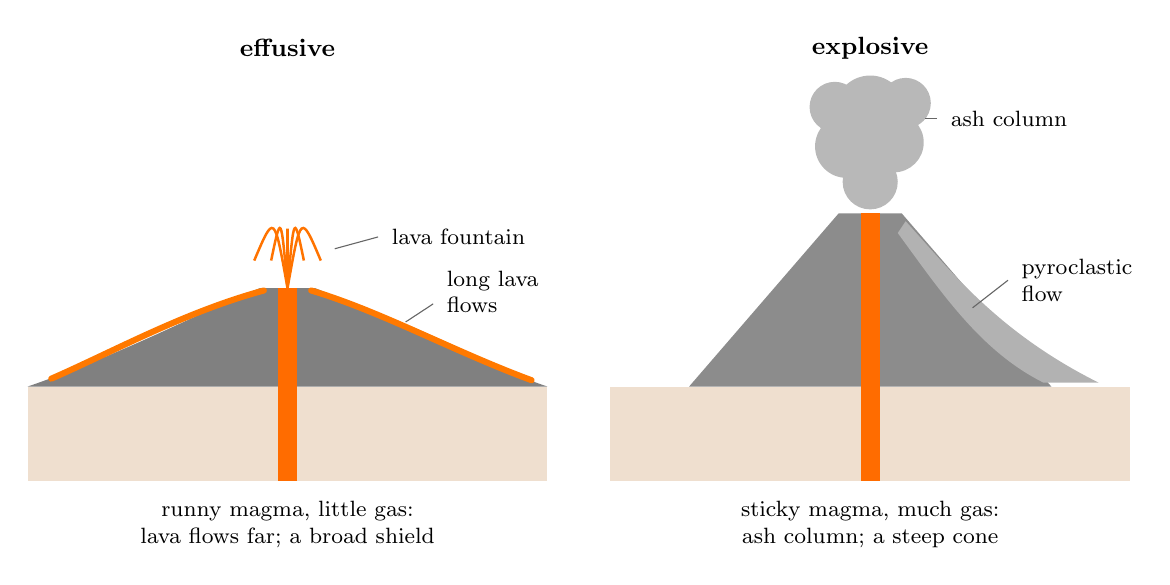
\begin{tikzpicture}[font=\small, x=1cm, y=1cm]
  % --- left: effusive, a shield
  \begin{scope}
    \fill[brown!25] (-3.3,-1.2) rectangle (3.3,0);
    \fill[black!50] (-3.3,0) .. controls (-2.0,0.45) and (-1.0,1.0) .. (-0.35,1.25)
      -- (0.35,1.25) .. controls (1.0,1.0) and (2.0,0.45) .. (3.3,0) -- cycle;
    \fill[orange!85!red] (-0.12,-1.2) rectangle (0.12,1.25);
    % fountain
    \foreach \a in {-25,-12,0,12,25}
      \draw[orange!90!red, line width=0.9pt] (0,1.25) .. controls ({0.4*sin(\a)},2.2) .. ({1.0*sin(\a)},1.6);
    % lava flows far down the gentle slopes
    \draw[orange!95!red, line width=2.2pt, line cap=round] (0.3,1.22) .. controls (1.2,0.95) and (2.1,0.45) .. (3.1,0.08);
    \draw[orange!95!red, line width=2.2pt, line cap=round] (-0.3,1.22) .. controls (-1.3,0.95) and (-2.2,0.45) .. (-3.0,0.1);
    \node[font=\small\bfseries] at (0,4.3) {effusive};
    \node[align=center, font=\footnotesize] at (0,-1.75) {runny magma, little gas:\\lava flows far; a broad shield};
    \node[anchor=west, font=\footnotesize] at (1.2,1.9) {lava fountain};
    \draw[black!60] (1.15,1.9) -- (0.6,1.75);
    \node[anchor=west, font=\footnotesize, align=left] at (1.9,1.2) {long lava\\flows};
    \draw[black!60] (1.85,1.05) -- (1.5,0.82);
  \end{scope}
  % --- right: explosive, a steep cone
  \begin{scope}[xshift=7.4cm]
    \fill[brown!25] (-3.3,-1.2) rectangle (3.3,0);
    \fill[black!45] (-2.3,0) -- (-0.4,2.2) -- (0.4,2.2) -- (2.3,0) -- cycle;
    \fill[orange!85!red] (-0.12,-1.2) rectangle (0.12,2.2);
    \foreach \x/\y/\r in {0/2.6/0.35, -0.3/3.05/0.4, 0.3/3.1/0.38, 0/3.5/0.45, -0.45/3.55/0.32, 0.45/3.6/0.32}
      \fill[black!28] (\x,\y) circle (\r);
    % pyroclastic flow down the flank
    \fill[black!30] (0.45,2.1) .. controls (1.0,1.5) and (1.6,0.7) .. (2.9,0.05)
      -- (2.2,0.05) .. controls (1.4,0.45) and (0.9,1.2) .. (0.35,1.95) -- cycle;
    \node[font=\small\bfseries] at (0,4.3) {explosive};
    \node[align=center, font=\footnotesize] at (0,-1.75) {sticky magma, much gas:\\ash column; a steep cone};
    \node[anchor=west, font=\footnotesize] at (0.9,3.4) {ash column};
    \draw[black!60] (0.85,3.4) -- (0.7,3.4);
    \node[anchor=west, font=\footnotesize, align=left] at (1.8,1.35) {pyroclastic\\flow};
    \draw[black!60] (1.75,1.35) -- (1.3,1.0);
  \end{scope}
\end{tikzpicture}

{\small The two kinds of \omterm{def:g4:volcanoes-earthquakes-first-look:eruption}{eruption} and the \omterm{def:g4:volcanoes-earthquakes-first-look:volcano}{volcanoes} they build (drawings,
not to scale).}
\label{fig:g7:volcanoes:two-kinds}
\end{omfigure}

\begin{method}[Effusive or explosive? Four clues]\label{met:g7:volcanoes:clues}
To tell from a description or a photograph which kind of \omterm{def:g4:volcanoes-earthquakes-first-look:eruption}{eruption} a \omterm{def:g4:volcanoes-earthquakes-first-look:volcano}{volcano}
has, look for these clues.
\begin{enumerate}
  \item \emph{What comes out?} \omterm{def:g4:volcanoes-earthquakes-first-look:eruption}{Lava} flowing or spurting in fountains:
        effusive. A column of ash, lumps of \omterm{def:g3:stones-pebbles-sand:rock}{rock} thrown out: explosive.
  \item \emph{The shape of the \omterm{def:g4:volcanoes-earthquakes-first-look:volcano}{volcano}.} A broad \omterm{def:g1:landscapes-around-us:landform}{mountain} with gentle
        slopes: mostly \omterm{def:g7:volcanoes:eruption-types}{effusive eruptions}. A steep cone: often explosive.
  \item \emph{The \omterm{def:g7:volcanoes:magma}{magma}.} Runny, little gas: effusive. Sticky, much gas:
        explosive.
  \item \emph{The \omterm{def:g3:stones-pebbles-sand:rock}{rocks} left behind.} Dark, solid \omterm{def:g4:volcanoes-earthquakes-first-look:eruption}{lava} flows: effusive.
        Layers of ash and pumice: explosive.
\end{enumerate}
\end{method}

\begin{example}[Using the clues]\label{ex:g7:volcanoes:clues}
A traveller describes a \omterm{def:g4:volcanoes-earthquakes-first-look:volcano}{volcano}: ``a huge, gently rounded \omterm{def:g1:landscapes-around-us:landform}{mountain}, black
\omterm{def:g4:volcanoes-earthquakes-first-look:eruption}{lava} flows everywhere on its slopes, some of them only a few years old''.
Clue~2 (gentle slopes) and clue~4 (dark \omterm{def:g4:volcanoes-earthquakes-first-look:eruption}{lava} flows) both point to \omterm{def:g7:volcanoes:eruption-types}{effusive
eruptions}: it is a shield \omterm{def:g4:volcanoes-earthquakes-first-look:volcano}{volcano}, like Mauna Loa.
\end{example}

\begin{inthelab}[A volcano in a bottle (in class, with the teacher)]
The teacher takes two closed bottles of fizzy water. One has been left
standing; the other has been gently shaken. Both are opened outdoors, over
a basin, pointing away from everyone. The still bottle hisses and lets a
few bubbles rise; the shaken one bursts into foam that shoots out. Which
bottle is like the \omterm{def:g7:volcanoes:magma}{magma} of Hawaii, which like Pinatubo's? Then drop a
piece of pumice and a \omterm{def:g3:stones-pebbles-sand:pebble}{pebble} into a bowl of water: the pumice floats. Look
at it through a magnifying glass: it is full of holes, the bubbles of gas
frozen into the \omterm{def:g3:stones-pebbles-sand:rock}{rock} as the \omterm{def:g7:volcanoes:magma}{magma} burst.
\end{inthelab}

\section{What comes out of a volcano}

An \omterm{def:g4:volcanoes-earthquakes-first-look:eruption}{eruption} throws out much more than \omterm{def:g4:volcanoes-earthquakes-first-look:eruption}{lava}: gases, ash, lumps of \omterm{def:g3:stones-pebbles-sand:rock}{rock} and,
in the worst cases, avalanches of hot ash.

The most abundant gas, by far, is water vapour. Large \omterm{def:g4:volcanoes-earthquakes-first-look:eruption}{eruptions} release
huge amounts of gas in a short time: on a single day of 1991, Pinatubo is
thought to have sent more than 250~million tonnes of gas into the upper
atmosphere.
% ledger: usgs:volcanic-gases

\begin{definition}[Pyroclastic flow]\label{def:g7:volcanoes:pyroclastic-flow}
A \emph{pyroclastic flow}\index{pyroclastic flow} is a fast avalanche of
hot gas, ash and pieces of \omterm{def:g3:stones-pebbles-sand:rock}{rock}, from grains of dust to boulders, which
rushes down the slopes of a \omterm{def:g4:volcanoes-earthquakes-first-look:volcano}{volcano} during an \omterm{def:g7:volcanoes:eruption-types}{explosive eruption}.
(\emph{Pyro} means fire and \emph{clastic} means made of broken pieces.)
\end{definition}

\omterm{def:g7:volcanoes:pyroclastic-flow}{Pyroclastic flows} usually move faster than \qty{80}{km/h}, and the \omterm{def:g3:stones-pebbles-sand:rock}{rocks}
and gas inside them are generally between 200 and \qty{700}{\degreeCelsius}.
They generally follow the \omterm{def:g1:landscapes-around-us:landform}{valleys}, like water, and knock down, burn or
bury nearly everything in their path. On 18~May 1980, the \omterm{def:g7:volcanoes:pyroclastic-flow}{pyroclastic flows} of Mount
St.~Helens raced at 80 to \qty{130}{km/h}, at a temperature of at least
\qty{700}{\degreeCelsius}, and reached \qty{8}{km} from the \omterm{def:g7:volcanoes:vent}{crater}.
% ledger: usgs:pyroclastic-flows, usgs:msh-flows, usgs:msh-reach

The table sums up the products of a \omterm{def:g4:volcanoes-earthquakes-first-look:volcano}{volcano}.

\begin{center}
\small
\begin{tabular}{|p{0.2\linewidth}|p{0.4\linewidth}|p{0.3\linewidth}|}
\hline
\textbf{product} & \textbf{what it is} & \textbf{the danger} \\
\hline
\omterm{def:g4:volcanoes-earthquakes-first-look:eruption}{lava} flow & molten \omterm{def:g3:stones-pebbles-sand:rock}{rock} flowing on the ground, then hardening & burns and buries what it meets, but usually slow enough for people to move out of the way \\
\hline
ash & tiny pieces of \omterm{def:g3:stones-pebbles-sand:rock}{rock} and glass, blown into the air & falls far away; roofs collapse under its weight; it damages aircraft \\
\hline
volcanic bombs & lumps of \omterm{def:g4:volcanoes-earthquakes-first-look:eruption}{lava} thrown out, which harden as they fly & crush what they hit, near the \omterm{def:g7:volcanoes:vent}{vent} \\
\hline
gases & mostly water vapour, then carbon dioxide and sulfur dioxide & some are poisonous; carbon dioxide gathers in hollows \\
\hline
\omterm{def:g7:volcanoes:pyroclastic-flow}{pyroclastic flow} & an avalanche of hot ash, \omterm{def:g3:stones-pebbles-sand:rock}{rock} and gas & the deadliest: too fast and too hot to escape \\
\hline
mudflow & ash and \omterm{def:g3:stones-pebbles-sand:rock}{rock} mixed with water from \omterm{def:g4:clouds-rain-snow:precipitation}{rain} or melted \omterm{def:g4:clouds-rain-snow:precipitation}{snow} & rushes down \omterm{def:g1:landscapes-around-us:landform}{valleys}, sometimes far from the \omterm{def:g4:volcanoes-earthquakes-first-look:volcano}{volcano} \\
\hline
\end{tabular}
\end{center}
% ledger: usgs:lava-flows, usgs:volcanic-gases, usgs:pyroclastic-flows, usgs:pinatubo-1991, usgs:msh-flows

\begin{method}[How long does it take?]\label{met:g7:volcanoes:time}
To find how long something moving at a known speed takes to cover a
distance, divide the distance by the speed:
\[
\text{time} = \frac{\text{distance}}{\text{speed}}.
\]
With a distance in kilometres and a speed in kilometres per hour, the time
comes out in hours; multiply by 60 to get minutes.
\end{method}

\begin{example}[Racing a pyroclastic flow]\label{ex:g7:volcanoes:race}
A \omterm{def:g7:volcanoes:pyroclastic-flow}{pyroclastic flow} moving at \qty{120}{km/h} heads for a village
\qty{6}{km} down the \omterm{def:g1:landscapes-around-us:landform}{valley}. It takes $6 \div 120 = 0.05$~hour, that is
$0.05 \times 60 = 3$~minutes. Three minutes: nobody can run, or even drive,
out of the \omterm{def:g1:landscapes-around-us:landform}{valley} in time. People are only safe if they have left
\emph{before} the \omterm{def:g4:volcanoes-earthquakes-first-look:eruption}{eruption}.
\end{example}

\begin{remark}[Mudflows: the danger that comes later]\label{rem:g7:volcanoes:mudflows}
% ledger: usgs:msh-flows, usgs:pinatubo-lahars
An \omterm{def:g4:volcanoes-earthquakes-first-look:eruption}{eruption} leaves the slopes covered with loose ash. When \omterm{def:g4:clouds-rain-snow:precipitation}{rain} falls on
it, or when the heat melts the \omterm{def:g4:clouds-rain-snow:precipitation}{snow} and ice of the summit, the ash turns
into mudflows that rush down the \omterm{def:g1:landscapes-around-us:landform}{valleys}. On 18~May 1980, the mudflows of
Mount St.~Helens damaged 27~bridges and nearly 200~homes. Around
Pinatubo, the heavy \omterm{def:g4:clouds-rain-snow:precipitation}{rains} of the following years turned the ash into
giant mudflows which buried whole villages: they did more damage than the
\omterm{def:g4:volcanoes-earthquakes-first-look:eruption}{eruption} itself.
\end{remark}


\section{Where are the volcanoes?}

The Smithsonian Institution, in Washington, keeps a list of all the
\omterm{def:g4:volcanoes-earthquakes-first-look:volcano}{volcanoes} known to have erupted in the last 12\,000 years: 1\,214 of them,
on land and under the \omterm{def:g2:water-on-earth:ocean}{sea}. For each one the list says where it
stands with respect to the \omterm{def:g7:plate-tectonics:plate}{plates}. The \omterm{def:g2:drawing-to-map:map}{map} below colours them in this way.
% ledger: data:gvp (counts computed in figdata/grade-7/volcano_settings.py)

\begin{omfigure}
\begin{tikzpicture}
\begin{axis}[ommap, width=\linewidth, xtick={-180,-90,...,180}, ytick={-60,0,60},
  legend style={at={(0.02,0.04)}, anchor=south west, font=\scriptsize,
  fill=white, fill opacity=0.85, text opacity=1, draw=black!40}, legend cell align=left]
\addplot[fill=omLithAlluv, draw=black!45, line width=0.2pt, forget plot] table {figdata/out/shared-geo-land.dat};
\addplot[omRidge!60, line width=0.5pt, forget plot] table {figdata/out/shared-geo-school-ridge.dat};
\addplot[omTrench!60, line width=0.5pt, forget plot] table {figdata/out/shared-geo-school-subduction.dat};
\addplot[only marks, mark=triangle*, mark size=1.3pt, omTrench, forget plot] table {figdata/out/grade-7-volcano_settings-map-sub.dat};
\addplot[only marks, mark=triangle*, mark size=1.3pt, omRidge, forget plot] table {figdata/out/grade-7-volcano_settings-map-rift.dat};
\addplot[only marks, mark=*, mark size=1.4pt, orange!90!black, forget plot] table {figdata/out/grade-7-volcano_settings-map-intra.dat};
\addlegendimage{only marks, mark=triangle*, mark size=1.6pt, omTrench}
\addlegendentry{where one plate sinks under another}
\addlegendimage{only marks, mark=triangle*, mark size=1.6pt, omRidge}
\addlegendentry{where plates move apart}
\addlegendimage{only marks, mark=*, mark size=1.6pt, orange!90!black}
\addlegendentry{inside a plate}
\end{axis}
\end{tikzpicture}

{\small The \omterm{def:g4:volcanoes-earthquakes-first-look:volcano}{volcanoes} active in the last 12\,000 years, coloured by where
they stand. Faint lines: the \omterm{def:g7:plate-tectonics:plate-boundary}{plate boundaries} where \omterm{def:g7:plate-tectonics:plate}{plates} move apart
(red) and where one \omterm{def:g7:plate-tectonics:plate}{plate} sinks under another (blue). Data: Smithsonian
Global Volcanism Program; boundaries after P.~Bird (2003); coastlines from
Natural Earth.}
% ledger: data:gvp, data:pb2002, data:ne-land
\label{fig:g7:volcanoes:map}
\end{omfigure}

\begin{omfigure}
\begin{tikzpicture}
  \begin{axis}[xbar, width=0.72\linewidth, height=3.6cm, bar width=8pt,
      xmin=0, xmax=1000, ymin=-0.6, ymax=3.6, y dir=reverse,
      ytick={0,...,3}, yticklabels from table={figdata/out/grade-7-volcano_settings.dat}{label},
      xlabel={number of volcanoes},
      axis x line=bottom, axis y line=left, axis line style={-},
      tick label style={font=\scriptsize}, label style={font=\small},
      nodes near coords, nodes near coords style={font=\scriptsize, anchor=west},
      point meta=explicit symbolic, enlarge y limits=false, clip=false]
    \addplot[fill=black!30, draw=black!60] table[x=n, y=idx, meta=n] {figdata/out/grade-7-volcano_settings.dat};
  \end{axis}
\end{tikzpicture}

{\small How many of the 1\,214 \omterm{def:g4:volcanoes-earthquakes-first-look:volcano}{volcanoes} stand in each setting.}
% ledger: data:gvp (figdata/grade-7/volcano_settings.py, main table)
\label{fig:g7:volcanoes:counts}
\end{omfigure}

\begin{proposition}[Most volcanoes stand on plate boundaries]\label{prop:g7:volcanoes:where}
% ledger: data:gvp (counts computed in figdata/grade-7/volcano_settings.py)
Of the 1\,214 \omterm{def:g4:volcanoes-earthquakes-first-look:volcano}{volcanoes} active in the last 12\,000 years, 838 (69~\%)
stand where one \omterm{def:g7:plate-tectonics:plate}{plate} sinks under another and 221 (18~\%) where \omterm{def:g7:plate-tectonics:plate}{plates}
move apart; 149 (12~\%) stand inside a \omterm{def:g7:plate-tectonics:plate}{plate}, far from its edges. For the
last 6 the setting is not known.
\end{proposition}

\textbf{Where \omterm{def:g7:plate-tectonics:plate}{plates} move apart.} Along the \omterm{def:g2:water-on-earth:ocean}{ocean} ridges, and in rifts such
as the one that is tearing East Africa apart, the \omterm{def:g7:plate-tectonics:plate}{plates} pull away from
each other. \omterm{def:g7:volcanoes:magma}{Magma} rises from the \omterm{def:g6:inside-the-earth:layers}{mantle} into the widening cracks and fills
them: new \omterm{def:g6:inside-the-earth:layers}{crust} is made. Most of the ridges lie under the \omterm{def:g2:water-on-earth:ocean}{sea}, but Iceland stands
right on the Mid-Atlantic Ridge: there, these \omterm{def:g4:volcanoes-earthquakes-first-look:volcano}{volcanoes} can be seen on
land. Their \omterm{def:g7:volcanoes:magma}{magma} is mostly runny basalt, and their \omterm{def:g4:volcanoes-earthquakes-first-look:eruption}{eruptions} are mostly
effusive.
% ledger: usgs:arc-magma, usgs:iceland, usgs:east-africa

\textbf{Where one \omterm{def:g7:plate-tectonics:plate}{plate} sinks under another.} More than two \omterm{def:g4:volcanoes-earthquakes-first-look:volcano}{volcanoes} in
three stand here, along lines that follow the edges of the Pacific \omterm{def:g2:water-on-earth:ocean}{Ocean}
--- the ``Ring of Fire'' --- and a few other places. Deep down, along the
sinking \omterm{def:g7:plate-tectonics:plate}{plate}, some of the \omterm{def:g3:stones-pebbles-sand:rock}{rock} partly melts; scientists still discuss
exactly which \omterm{def:g3:stones-pebbles-sand:rock}{rock} melts, the sinking \omterm{def:g7:plate-tectonics:plate}{plate} or the \omterm{def:g7:plate-tectonics:plate}{plate} above it, or both.
The \omterm{def:g7:volcanoes:magma}{magma} that rises there is often sticky and full of gas: these are the
explosive \omterm{def:g4:volcanoes-earthquakes-first-look:volcano}{volcanoes}, like Mount St.~Helens and Pinatubo. The data show it:
of the 660 steep cones (stratovolcanoes) in the list, 564 --- that is
85~\% --- stand where one \omterm{def:g7:plate-tectonics:plate}{plate} sinks under another.
% ledger: usgs:arc-magma, data:gvp (figdata/grade-7/volcano_settings.py, part strato)

\textbf{Inside a \omterm{def:g7:plate-tectonics:plate}{plate}.} A few \omterm{def:g4:volcanoes-earthquakes-first-look:volcano}{volcanoes} are far from any boundary. The
most famous are those of Hawaii, in the middle of the Pacific \omterm{def:g2:water-on-earth:ocean}{Ocean}, more
than \qty{3200}{km} from the nearest edge of a \omterm{def:g7:plate-tectonics:plate}{plate}.
% ledger: usgs:hawaii-hotspot

\begin{definition}[Hotspot]\label{def:g7:volcanoes:hotspot}
A \emph{hotspot}\index{hotspot} is a place, deep in the \omterm{def:g6:inside-the-earth:layers}{mantle}, which
stays hot for millions of years and keeps feeding \omterm{def:g7:volcanoes:magma}{magma} to \omterm{def:g4:volcanoes-earthquakes-first-look:volcano}{volcanoes} at
the surface, even far from the edges of the \omterm{def:g7:plate-tectonics:plate}{plates}.
\end{definition}

The \omterm{def:g7:volcanoes:hotspot}{hotspot} stays where it is, while the \omterm{def:g7:plate-tectonics:plate}{plate} above it moves. A \omterm{def:g4:volcanoes-earthquakes-first-look:volcano}{volcano}
grows above the \omterm{def:g7:volcanoes:hotspot}{hotspot}; then the moving \omterm{def:g7:plate-tectonics:plate}{plate} carries it away, and it
dies, while a new \omterm{def:g4:volcanoes-earthquakes-first-look:volcano}{volcano} grows over the \omterm{def:g7:volcanoes:hotspot}{hotspot} behind it. In time, the
\omterm{def:g7:plate-tectonics:plate}{plate} carries a whole line of \omterm{def:g4:volcanoes-earthquakes-first-look:volcano}{volcanoes}, the oldest farthest from the
\omterm{def:g7:volcanoes:hotspot}{hotspot}. That is just what we see in Hawaii: the oldest \omterm{def:g3:stones-pebbles-sand:rock}{rocks} of the
island of Kauai, at the north-west end of the inhabited islands, are about
5.5~million years old, and deeply worn down by \omterm{def:g4:clouds-rain-snow:precipitation}{rain} and waves; on the Big
Island, at the south-east end, the oldest \omterm{def:g3:stones-pebbles-sand:rock}{rocks} at the surface are less
than 0.7~million years old, and new \omterm{def:g4:volcanoes-earthquakes-first-look:eruption}{lava} still comes out.
% ledger: usgs:hawaii-hotspot

\begin{history}[A geophysicist and a line of islands]
% ledger: usgs:hawaii-hotspot
Why should a chain of volcanic islands rise in the middle of the largest
\omterm{def:g7:plate-tectonics:plate}{plate} on Earth? In 1963 the Canadian geophysicist J.~Tuzo Wilson proposed
an answer. The Hawaiian islands, he suggested, are a line because the
Pacific \omterm{def:g7:plate-tectonics:plate}{plate} moves over a deep, fixed source of heat in the \omterm{def:g6:inside-the-earth:layers}{mantle}, which
partly melts the \omterm{def:g7:plate-tectonics:plate}{plate} above it. If he was right, the islands should be
older and more worn down the farther they are from the active \omterm{def:g4:volcanoes-earthquakes-first-look:volcano}{volcanoes} of
the Big Island. The ages of their \omterm{def:g3:stones-pebbles-sand:rock}{rocks} show exactly that. A single idea explained both the line and the order of the ages.
(Wilson is also the scientist who discovered the \omterm{def:g7:plate-tectonics:plate-boundary}{transform boundaries},
where \omterm{def:g7:plate-tectonics:plate}{plates} slide past each other.)
\end{history}

\begin{omfigure}
\begin{tikzpicture}[font=\small, x=1cm, y=1cm]
  % sea, plate and mantle
  \fill[omSea!45] (-6.2,0) rectangle (6.2,1.0);
  \fill[orange!12] (-6.2,-3.4) rectangle (6.2,-1.0);
  \fill[brown!35] (-6.2,-1.0) rectangle (6.2,0);
  \draw[omSea!80!black, line width=0.5pt] (-6.2,1.0) -- (6.2,1.0);
  \node[font=\footnotesize] at (-4.6,-0.5) {Pacific plate};
  % the hotspot plume, fixed in the mantle, and the magma rising to the volcano
  \fill[orange!80!red] (4.0,-3.4) .. controls (3.6,-2.4) .. (3.75,-1.0) -- (4.25,-1.0) .. controls (4.4,-2.4) .. (4.0,-3.4) -- cycle;
  \node[anchor=west, align=left, font=\footnotesize] at (4.5,-2.5) {hotspot: stays\\in place};
  % volcanoes rise from the sea floor; youngest over the hotspot
  \fill[black!55] (2.3,0) .. controls (3.2,1.2) .. (3.75,1.85) -- (4.25,1.85) .. controls (4.8,1.2) .. (5.7,0) -- cycle;
  \fill[orange!80!red] (3.93,-1.0) rectangle (4.07,1.85);
  \fill[black!45] (-0.4,0) .. controls (0.4,0.9) .. (0.9,1.3) -- (1.3,1.3) .. controls (1.8,0.9) .. (2.6,0) -- cycle;
  \fill[black!35] (-3.2,0) .. controls (-2.5,0.6) .. (-2.1,0.8) -- (-1.7,0.8) .. controls (-1.3,0.6) .. (-0.6,0) -- cycle;
  \fill[black!28] (-5.8,0) .. controls (-5.2,0.4) .. (-4.9,0.5) -- (-4.6,0.5) .. controls (-4.3,0.4) .. (-3.6,0) -- cycle;
  % labels
    \node[align=center, font=\footnotesize, anchor=south] at (4.3,1.95) {active volcano\\(Big Island: less\\than 0.7 million years)};
  \node[align=center, font=\footnotesize, anchor=south] at (0.7,1.4) {old, worn-down island\\(Kauai: about\\5.5 million years)};
  \node[align=center, font=\footnotesize] at (-1.9,1.5) {older volcano,\\below the waves};
  \node[align=center, font=\footnotesize] at (-4.75,1.3) {still older,\\sinking};
  \node[font=\footnotesize] at (5.75,0.55) {sea};
  \node[font=\footnotesize] at (-4.3,-2.2) {mantle};
  % plate motion
  \draw[-{Stealth[length=3mm]}, line width=1.2pt] (2.2,-0.62) -- (-1.8,-0.62);
  \node[font=\footnotesize] at (0.2,-0.28) {the plate moves north-west};
    \node[font=\footnotesize\bfseries] at (-5.8,-3.1) {NW};
  \node[font=\footnotesize\bfseries] at (5.8,-3.1) {SE};
\end{tikzpicture}

{\small A \omterm{def:g7:plate-tectonics:plate}{plate} moving over a \omterm{def:g7:volcanoes:hotspot}{hotspot} (a drawing, not to scale; the islands
in between are left out). The \omterm{def:g4:volcanoes-earthquakes-first-look:volcano}{volcano} over the \omterm{def:g7:volcanoes:hotspot}{hotspot} is young and
active; the \omterm{def:g7:plate-tectonics:plate}{plate} carries the older ones away to the north-west, where
they die, wear down and finally sink below the waves.}
% ledger: usgs:hawaii-hotspot
\label{fig:g7:volcanoes:hotspot}
\end{omfigure}

\begin{omfigure}
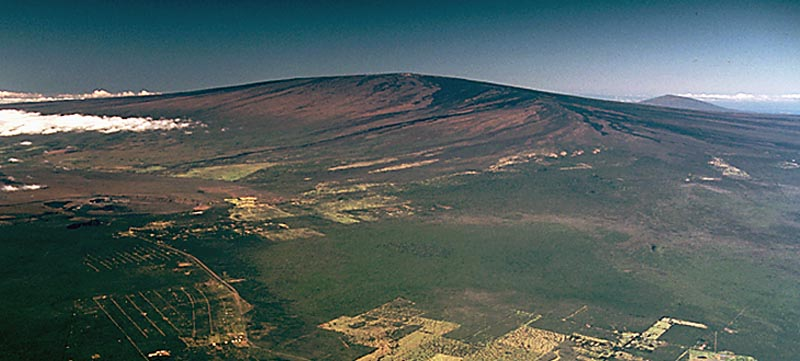
\includegraphics[width=0.8\linewidth]{images/book1/g7-mauna-loa.jpg}

{\small Mauna Loa, a shield \omterm{def:g4:volcanoes-earthquakes-first-look:volcano}{volcano} on the Big Island of Hawaii, seen from
the air: a huge \omterm{def:g1:landscapes-around-us:landform}{mountain} with gentle slopes, built by thousands of runny
\omterm{def:g4:volcanoes-earthquakes-first-look:eruption}{lava} flows. Photograph: J.~D. Griggs, U.S. Geological Survey, 1985 (public
domain, via Wikimedia Commons).}
% ledger: commons:mauna-loa
\label{fig:g7:volcanoes:mauna-loa}
\end{omfigure}

\section{Living with volcanoes}

Many people live near \omterm{def:g4:volcanoes-earthquakes-first-look:volcano}{volcanoes}: about 3~million lived in the region
around Pinatubo in 1991. Luckily, a large \omterm{def:g4:volcanoes-earthquakes-first-look:eruption}{eruption} often gives warning
signs. Rising \omterm{def:g7:volcanoes:magma}{magma} pushes the \omterm{def:g3:stones-pebbles-sand:rock}{rocks} aside: the ground cracks and
shakes with small \omterm{def:g4:volcanoes-earthquakes-first-look:earthquake}{earthquakes}, the slopes swell, gas escapes. At Mount
St.~Helens, the first small \omterm{def:g4:volcanoes-earthquakes-first-look:earthquake}{earthquakes} came on 16~March 1980; by 17~May
there had been more than 10\,000, and the north side had swollen outwards
by at least \qty{137}{m}. Scientists measured all this and the area was
closed; even so, 57~people died on 18~May.
% ledger: usgs:msh-lead-up, usgs:msh-flows

At Pinatubo, in 1991, the scientists who watched the \omterm{def:g4:volcanoes-earthquakes-first-look:earthquake}{earthquakes}, the gas
and the swelling of the \omterm{def:g4:volcanoes-earthquakes-first-look:volcano}{volcano} gave the warning in time: people living
near the \omterm{def:g4:volcanoes-earthquakes-first-look:volcano}{volcano} left, and at least 5\,000 lives were saved.
% ledger: usgs:pinatubo-1991 (central Luzon home to about 3 million people)

\begin{remark}[Never go near an erupting volcano]\label{rem:g7:volcanoes:safety}
Watching an \omterm{def:g4:volcanoes-earthquakes-first-look:eruption}{eruption} is only for the places that the authorities have
opened to the public. Gases, falling \omterm{def:g3:stones-pebbles-sand:rock}{rocks}, fresh lava crust that breaks
under your feet and \omterm{def:g7:volcanoes:pyroclastic-flow}{pyroclastic flows} can kill, often without warning.
\omterm{def:g4:volcanoes-earthquakes-first-look:volcano}{Volcano} observatories publish what is safe to visit: always follow them.
\end{remark}

\section{Exercises}

\begin{exercise}[$\star$]\label{exo:g7:volcanoes:1}
Match each word with its meaning: \omterm{def:g7:volcanoes:magma}{magma}; \omterm{def:g4:volcanoes-earthquakes-first-look:eruption}{lava}; \omterm{def:g7:volcanoes:magma-chamber}{magma chamber}; \omterm{def:g7:volcanoes:vent}{vent};
\omterm{def:g7:volcanoes:vent}{crater}. (a) A bowl-shaped hollow at the top of a \omterm{def:g4:volcanoes-earthquakes-first-look:volcano}{volcano}. (b) Molten \omterm{def:g3:stones-pebbles-sand:rock}{rock}
underground. (c) An opening through which \omterm{def:g7:volcanoes:magma}{magma} comes out. (d) Molten \omterm{def:g3:stones-pebbles-sand:rock}{rock}
that has come out at the surface. (e) A large pocket of \omterm{def:g7:volcanoes:magma}{magma} a few
kilometres under a \omterm{def:g4:volcanoes-earthquakes-first-look:volcano}{volcano}.
\end{exercise}

\begin{exercise}[$\star$]\label{exo:g7:volcanoes:2}
Effusive or explosive? (a) \omterm{def:g1:landscapes-around-us:water}{Rivers} of glowing \omterm{def:g4:volcanoes-earthquakes-first-look:eruption}{lava} flow down a gentle
slope. (b) A column of ash rises \qty{35}{km} into the sky. (c) A
fountain of glowing drops spurts from a crack. (d) An avalanche of hot ash
and gas rushes down a \omterm{def:g1:landscapes-around-us:landform}{valley}.
\end{exercise}

\begin{exercise}[$\star$]\label{exo:g7:volcanoes:3}
True or false? Correct the false ones. (a) \omterm{def:g7:volcanoes:magma}{Magma} and \omterm{def:g4:volcanoes-earthquakes-first-look:eruption}{lava} are two names of
the same molten \omterm{def:g3:stones-pebbles-sand:rock}{rock}, underground and at the surface. (b) The most
abundant volcanic gas is carbon dioxide. (c) A \omterm{def:g7:volcanoes:pyroclastic-flow}{pyroclastic flow} is a \omterm{def:g1:landscapes-around-us:water}{river}
of liquid \omterm{def:g4:volcanoes-earthquakes-first-look:eruption}{lava}. (d) The Hawaiian \omterm{def:g4:volcanoes-earthquakes-first-look:volcano}{volcanoes} stand on a \omterm{def:g7:plate-tectonics:plate-boundary}{plate boundary}.
\end{exercise}

\begin{exercise}[$\star$]\label{exo:g7:volcanoes:4}
Use the table of glow colours. (a) \omterm{def:g4:volcanoes-earthquakes-first-look:eruption}{Lava} glows yellow: give its
temperature. (b) A hardening flow glows dark red: give its temperature.
(c) A photograph shows orange \omterm{def:g4:volcanoes-earthquakes-first-look:eruption}{lava} at the front of a flow and yellow \omterm{def:g4:volcanoes-earthquakes-first-look:eruption}{lava}
near the \omterm{def:g7:volcanoes:vent}{vent}. Where is it hotter? Why?
\end{exercise}

\begin{exercise}[$\star\star$]\label{exo:g7:volcanoes:5}
Use the bar chart of the 1\,214 \omterm{def:g4:volcanoes-earthquakes-first-look:volcano}{volcanoes}. (a) How many \omterm{def:g4:volcanoes-earthquakes-first-look:volcano}{volcanoes} stand on
a \omterm{def:g7:plate-tectonics:plate-boundary}{plate boundary} (where \omterm{def:g7:plate-tectonics:plate}{plates} move apart, or where one sinks under
another)? (b) What percentage of all the \omterm{def:g4:volcanoes-earthquakes-first-look:volcano}{volcanoes} is that? (c) Check that
the four percentages of the proposition add up to about 100~\%.
\end{exercise}

\begin{exercise}[$\star\star$]\label{exo:g7:volcanoes:6}
Of the 660 steep cones (stratovolcanoes) of the list, 564 stand where one
\omterm{def:g7:plate-tectonics:plate}{plate} sinks under another, 62 where \omterm{def:g7:plate-tectonics:plate}{plates} move apart and 33 inside a
\omterm{def:g7:plate-tectonics:plate}{plate}. (a) Find the percentage of steep cones that stand where one \omterm{def:g7:plate-tectonics:plate}{plate}
sinks under another. (b) How many steep cones are left for the setting ``not
known''? (c) Use the four clues: what kind of \omterm{def:g4:volcanoes-earthquakes-first-look:eruption}{eruptions} should we expect
along the Ring of Fire?
\end{exercise}

\begin{exercise}[$\star\star$]\label{exo:g7:volcanoes:7}
At Kilauea, \omterm{def:g4:volcanoes-earthquakes-first-look:eruption}{lava} leaves the \omterm{def:g7:volcanoes:vent}{vent} at about \qty{1170}{\degreeCelsius}. In a
\omterm{def:g4:volcanoes-earthquakes-first-look:eruption}{lava} tunnel it reached the \omterm{def:g2:water-on-earth:ocean}{sea}, \qty{10}{km} away, at about
\qty{1140}{\degreeCelsius}. (a) By how many degrees did it cool? (b) How
many degrees is that per kilometre? (c) \omterm{def:g4:volcanoes-earthquakes-first-look:eruption}{Lava} in the open air cools by
hundreds of degrees per second at its surface. Explain why the \omterm{def:g4:volcanoes-earthquakes-first-look:eruption}{lava} in
the tunnel stayed so hot.
\end{exercise}

\begin{exercise}[$\star\star$]\label{exo:g7:volcanoes:8}
The oldest \omterm{def:g3:stones-pebbles-sand:rock}{rocks} of Kauai are about 5.5~million years old; those of the Big
Island, less than 0.7~million years old. (a) Which island is older? By at
least how many million years? (b) Which island is more worn down? Why?
(c) Which island stands over the \omterm{def:g7:volcanoes:hotspot}{hotspot} today? (d) Kauai lies north-west
of the Big Island. In which direction does the Pacific \omterm{def:g7:plate-tectonics:plate}{plate} carry the
islands?
\end{exercise}

\begin{exercise}[$\star\star$]\label{exo:g7:volcanoes:9}
The Hawaiian islands are more than \qty{3200}{km} from the nearest \omterm{def:g7:plate-tectonics:plate-boundary}{plate
boundary}. (a) Why is that surprising for \omterm{def:g4:volcanoes-earthquakes-first-look:volcano}{volcanoes}? (b) Explain in three or
four sentences where their \omterm{def:g7:volcanoes:magma}{magma} comes from. (c) On the \omterm{def:g2:drawing-to-map:map}{map} of the
\omterm{def:g4:volcanoes-earthquakes-first-look:volcano}{volcanoes}, which colour are they?
\end{exercise}

\begin{exercise}[$\star\star$]\label{exo:g7:volcanoes:10}
In June~1991 the first \omterm{def:g7:volcanoes:magma}{magma} of Pinatubo oozed out quietly; three days
later, other \omterm{def:g7:volcanoes:magma}{magma} exploded. Using the two bottles of fizzy water, explain
the difference. Which of the two \omterm{def:g7:volcanoes:magma}{magmas} had lost its gas on the way up?
\end{exercise}

\begin{exercise}[$\star\star\star$]\label{exo:g7:volcanoes:11}
A village stands \qty{10}{km} down a \omterm{def:g1:landscapes-around-us:landform}{valley} from a \omterm{def:g4:volcanoes-earthquakes-first-look:volcano}{volcano}. (a) A
\omterm{def:g7:volcanoes:pyroclastic-flow}{pyroclastic flow} moves at \qty{80}{km/h}. How many minutes would it take
to reach the village? (b) Same question at \qty{130}{km/h}. (c) A family
needs 20~minutes to leave by car. Explain why the warning has to come
before the \omterm{def:g4:volcanoes-earthquakes-first-look:eruption}{eruption} starts, not when the flow is seen.
\end{exercise}

\begin{exercise}[$\star\star\star$]\label{exo:g7:volcanoes:12}
The ash of Mount St.~Helens went once around the whole Earth in 15~days.
One degree of \omterm{def:g6:latitude-longitude:latitude}{latitude} is about \qty{111}{km}, and a full turn is
360~degrees. (a) About how long is a full turn of the Earth, in
kilometres? Round to the nearest thousand. (b) How many kilometres did
the ash travel per day, on average? (c) How many kilometres per hour is
that? (d) Is the ash carried by the wind or by its own speed? Explain.
% ledger: usgs:msh-may18, rmg:latitude-def
\end{exercise}

\section{Problem: The day the mountain lost its top}

\begin{problem}[{Weekend problem --- the warning signs of Mount St.~Helens,
the eruption of 18~May 1980, and how much of the mountain was gone}]
\label{pb:g7:volcanoes:1}
% ledger: usgs:msh-heights, usgs:msh-lead-up, usgs:msh-may18, usgs:msh-flows, usgs:msh-reach, usgs:msh-dome, usgs:msh-faq-loss, data:gvp, tht:everest

Mount St.~Helens stands in the north-west of the United States. Use the
photographs at the start of the chapter, the \omterm{def:g2:drawing-to-map:map}{map} of the \omterm{def:g4:volcanoes-earthquakes-first-look:volcano}{volcanoes} and the
numbers below, measured by the U.S. Geological Survey.

\medskip
\noindent\textbf{Part I --- Before the eruption.}
\begin{enumerate}
  \item The first small \omterm{def:g4:volcanoes-earthquakes-first-look:earthquake}{earthquakes} came on 16~March 1980; the great
        \omterm{def:g4:volcanoes-earthquakes-first-look:eruption}{eruption} on 18~May. How many days passed between the two? (March
        has 31~days, April~30.)
  \item By 17~May, more than 10\,000 \omterm{def:g4:volcanoes-earthquakes-first-look:earthquake}{earthquakes} had been recorded,
        in the 62~days since 16~March. About how many is that per day, on
        average?
  \item The north side of the \omterm{def:g1:landscapes-around-us:landform}{mountain} swelled outwards by at least
        \qty{137}{m}. Explain why the swelling worried the scientists.
  \item On the \omterm{def:g2:drawing-to-map:map}{map} of the \omterm{def:g4:volcanoes-earthquakes-first-look:volcano}{volcanoes}, Mount St.~Helens is a blue triangle.
        What does that tell you about its setting? Which kind of \omterm{def:g4:volcanoes-earthquakes-first-look:eruption}{eruption}
        do you expect, and which shape of \omterm{def:g4:volcanoes-earthquakes-first-look:volcano}{volcano}?
\end{enumerate}

\medskip
\noindent\textbf{Part II --- 18 May 1980.}\par\nopagebreak
\begin{enumerate}[resume, beginpenalty=10000]
  \item At 8:32 a small \omterm{def:g4:volcanoes-earthquakes-first-look:earthquake}{earthquake} set the swollen side sliding. The
        \omterm{def:g5:natural-hazards:landslide}{landslide} moved at up to \qty{240}{km/h}. How many kilometres is
        that per minute?
  \item The \omterm{def:g5:natural-hazards:landslide}{landslide} uncovered the \omterm{def:g7:volcanoes:magma}{magma} like a cork pulled from a shaken
        bottle. Explain why the \omterm{def:g4:volcanoes-earthquakes-first-look:volcano}{volcano} then exploded sideways.
  \item The sideways blast moved at least \qty{480}{km/h} and reached
        \qty{27}{km} from the \omterm{def:g4:volcanoes-earthquakes-first-look:volcano}{volcano}. At that speed, how many minutes did
        it take, at most, to get there?
  \item The \omterm{def:g7:volcanoes:pyroclastic-flow}{pyroclastic flows} moved at up to \qty{130}{km/h} and reached
        \qty{8}{km} from the \omterm{def:g7:volcanoes:vent}{crater}. How many minutes did they take at that
        speed? Round to the nearest minute.
\end{enumerate}

\medskip
\noindent\textbf{Part III --- After.}\par\nopagebreak
\begin{enumerate}[resume, beginpenalty=10000]
  \item The column of ash reached a height of about \qty{24}{km} in less
        than 15~minutes. How many times higher than Mount Everest
        (\qty{8.8}{km}) is that? Round to one decimal.
  \item Between 1980 and 1986, sticky \omterm{def:g4:volcanoes-earthquakes-first-look:eruption}{lava} oozed out in the \omterm{def:g7:volcanoes:vent}{crater} and
        built a mound \qty{267}{m} high over the \omterm{def:g7:volcanoes:vent}{vent}. Were these
        \omterm{def:g4:volcanoes-earthquakes-first-look:eruption}{eruptions} effusive or explosive? Which bottle of fizzy water do
        they remind you of?
  \item Look at the two photographs of the \omterm{def:g4:volcanoes-earthquakes-first-look:volcano}{volcano}. Describe in two
        sentences what changed.
  \item Before the \omterm{def:g4:volcanoes-earthquakes-first-look:eruption}{eruption}, the summit was \qty{2950}{m} above \omterm{def:g4:world-physical-map:altitude}{sea level};
        after it, the highest point was \qty{2549}{m}. How many metres of
        height did the \omterm{def:g1:landscapes-around-us:landform}{mountain} lose?
\end{enumerate}
\end{problem}
